\mysection{The Night Child}{species-night-child}

\flavor{
"Lie close," Laura said, \\
Pricking up her golden head:\\
"We must not look at goblin men,\\
We must not buy their fruits:\\
Who knows upon what soil they fed\\
Their hungry thirsty roots?"\\
\Tilde "Goblin Market", Christina Rossetti

}

\begin{center}
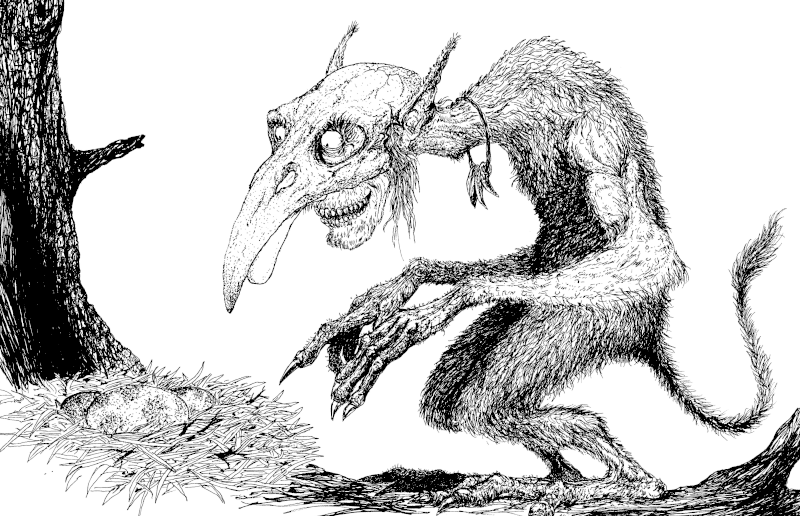
\includegraphics[width=\linewidth,keepaspectratio=true]{species/NightChildren2}
\end{center}



\mysubsection{Appearance}{night-child-appearance}

You are a child of \mylink{the Void}{the-void}, a creature of pure Chaos intruding in the Dream like a splinter in a finger. Your appearance and abilities are completely random, as numerous and varied as the fungus of the woods. No one knows how the Night Children are born, or where they come from - where they gain their talents, or how they arrive in reality carrying magical and wondrous treasures. The Night Children cover every continent and nation, and can be found in odd and unlikely places where you least expect them. 

While you aren't the social pariahs that the Rom (Murks and Spriggans) are, Mortals find you kind of weird and gross (though still likable). They certainly don't invite you into fine establishments, and generally think you're pretty stupid before they even get to know you.  You get the impression that Mortals think of you as a really ugly and dumb dog - they tolerate you fine, but when push comes to shove they don't think of you on the same "level" as they are.

Mortals won't direct questions to you if there are other Mortals in your Band present, and will generally try to ignore your antics (like a drunk on a subway). Mortals also know that you are \myital{extremely} strong and tough, however - so they won't provoke you or start fights if they can help it.




\begin{multicols*}{2}\raggedcolumns

\mysubsection{Virtues}{night-child-virtues-basic}

\myhighlight{Undreamt}{night-child-virtue-undreamt}

You stand outside of the Dream and are thus untouched by Sish, the Handmaiden of Time. You are immune to aging of any kind, and your \DEATH starts at Tough (d4).


\mysubsection{Complications}{night-child-complications}

\myhighlight{No Talk Good!}{night-child-complication-no-talk-good}

You can only speak in words of 2 syllables or fewer.

\myhighlight{Tiny}{night-child-complication-tiny}
  
You stand only 1m tall to start.  You can only carry a \mypg{Burden}{gear-burden} equal to your \VIG (you don't get the +2 bonus). If you wear armor, you can only wear armor for "little people" (child-sized).  You cannot wield 2-handed weapons.

  \myhighlight{Unseelie}{night-child--complication-unseelie}
    
  You are creature of Chaos, one of the \mylink{Unseelie}{the-inhabitants} - and are thus \mybold{Unhallowed}.

  \mysubsection{Starting Gear}{night-child-starting-gear}

    In addition to your Gear roll, you have:

  \callout{
    \mybullet {
      \item a half pair of scissors (treat as a \mylink{Dagger}{gear-dex-weapons}) or a big stick (treat as a \mylink{Club}{gear-vig-weapons});
      \item \UDD{d4} of \mylink{Personal Provisions}{gear-equipment};
      \item 5 useless items (wad of used tissues, taxidermied toad, etc)
    }}


\cbreak

\myimage{species/NightChildren4}


  \mysubsection{Creation}{night-child-creation}

  \callout {
    \footnotesize{
        \mynumlist {
            \item You start with \mybold{8 Flesh and 2 Grit}. 
            \item Move your \TAL \DCUP (to a d6). If you need to \RSTRY{\TAL}, you only fail on a natural 1 (instead of a 1 or 2). Put a check next to \TAL on your \mylink{Adventurer Sheet}{adventurer-sheet.8} so you don't forget.
            \item Write down your starting \mylink{Virtues}{night-child-virtues} and \mylink{Complications}{night-child-complications}.
            \item Roll 3d6 to determine your Weird, Looks, Gear, and Snag. See the section \mylink{Make Me!}{night-child-virtues} below.
            \item Write down your \mylink{Starting Gear}{night-child-starting-gear}.
        }
    }
  }

Night Children are "special" in that some of their Virtues and Complications are completely random. Grab 3d6 and follow the directions under the \mylink{Make Me!}{night-child-virtues} section on the next page.



\end{multicols*}

  \newpage


  \mysubsection{Make Me!}{night-child-virtues}

  Roll 3d6.  Apply the result of one of the dice to a \mylink{Weird Virtue}{night-children-virtues-weird}, a second to a \mylink{Looks Virtue}{night-children-virtues-looks}, and the final die to a \mylink{Gear Virtue}{night-children-virtues-gear}.  The \SUM of the dice determines your \mylink{Snag}{night-children-complications}.



  \mytable{c X X X}{
    \thead{Roll} & \thead{Weird} & \thead{Looks} & \thead{Gear} \\
}{
        1 & Bug Barf & Fishy & Bedlam Bag \\
        2 & Crafty & Glass Teeth & Big Helm \\
        3 & Gassy & Owl Head & Big Shield \\
        4 & Run Away & Rat Tail & Bug Pal \\
        5 & Shocky & Spider Eyes & Devil Pen \\
        6 & Spin Silk & Sticky & Gobbomb \\
        7 & Anklebiter  & Bat Ears & Gobsword \\
        8 & Twitchy & Tusky & Trunk Pal \\
        9 & Bad Blood & Frog Mouth & Little Buddy \\
        10 & Shedding & Pig Snout & Skelly Key \\
        11 & Bad Spit & Harpy Claws & Big Pal \\
        12 & Rando & Rooty & Gremlin Tools \\
        13 & Bloodthirst & Bigg'un & Bogeylatch \\
        14 & Bouncy & Camo & Kazoo \\
        15 & Crazy & Skin Bag & Magic Beans \\
        16 & Meat on Menu & Tough'un & Mirror Mirror \\
        17 & Big Boom & Fly Wings & Hole \\
        18 & Eat Brains & Goo & Kissy Lips \\
        19 & Nose Hairs & 'nother Arm & Red Shoes \\
        20 & Wut? & Shell & Spinny Wheel \\
        21 & Bad Breath & Babies! & Fly Rug \\
        22 & Go Night Night & Beardy & Packpack \\
        23 & Troll Blood &  Smoky & The Crew \\
        24 & Me Human! & Lie Can & Vorpal Sword \\ 
}

  \mybold{Snags} (total of Weird, Looks, and Gear)

  \mytable{c X l X l X}{
    \thead{Roll} & \thead{} & \thead{Roll} & \thead{} & \thead{Roll} & \thead{} \\
}{
      3 & Angry & 9 & Glowy & 15 & Smell Yummy \\
      4 & Backwards & 10 & Me Cold! & 16 & Stealy \\
      5 & Bad Mouth & 11 & Me Hot! & 17 & Weird Voice \\
      6 & Bumpback & 12 & Me Hungry! & 18 & Who Dat? \\
      7 & Dirty & 13 & Me Tired ... & - & - \\
      8 & Fat & 14 & Pinhead & - & - \\
}
      

  \callout {
    Weird and Looks get more powerful the more times you roll the result. See the description for details.
    \myskip
    Gear is unique.  If you roll a result you've rolled before, roll again.
}


\newpage
\begin{multicols*}{2}\raggedcolumns
\mysubsection{Weird}{night-children-virtues-weird}



\callout {
    Weird Virtues get more powerful the more times you roll the result. See the description for details.
}


\NC[Name=Anklebiter]

\mybold{1st time:} You deal +1 damage.

\mybold{2nd time:} You deal +2 damage.

\mybold{3rd time:} You deal +4 damage.

\mybold{4th or more:} Roll again.


\NC[Name=Bad Blood]

\mybold{1st time:} Your blood is acidic and, if you choose, can be made to spray in a really gross and weird way if you're cut. Every time you take damage to your Flesh, you can force everyone (including Allies) Close to try their \SAVE{Doom} or be sprayed with \mylink{Acid}{malignants-acids} (see the section on \mylink{Malignants}{research-chymistry-malignants} under \mypg{Research: Chymistry}{research-chymistry}). You can only choose one of the three possible effects of an Acid. Again, you can choose whether or not your blood sprays everywhere, unless you are affected by \effect{Bleeding}.

\mybold{2nd time:} As above, but choose up to 2 effects, and the spray reaches all creatures Close and Nearby.


\mybold{3rd time:} As above, but choose up to 3 effects, and the spray reaches all creatures Close, Nearby, and Distant.


\mybold{4th or more:} Roll again.


\cbreak

\NC[Name=Bad Breath]

\mybold{1st time:} Once per Session, you can breathe out a cone of fire, acid, frost, etc (your choice).  The breath does 3d6 damage, \SAVE{Doom} for half damage.

\mybold{2nd time:} As above, but you deal 5d6 damage.

\mybold{3rd time:} As above, but you deal \LVL d6 damage.

\mybold{4th or more:} Roll again.


\NC[Name=Bad Spit]

\mybold{1st time:} You have a few toxic sacs somewhere in your head. Once per Session, you can drool out \UDD{d2} of a \mylink{Noxious (d6) Toxin}{malignants-toxins} that can be collected (treat as an Unguent), spit onto a blade, etc.   Once per Session, you can spit out a dram or so of liquid that acts as an Iron toxin.  Treat this toxin as an Unguent.

\mybold{2nd time:} As above, but you can choose to spit this toxin at someone Close (treat as an \INT weapon) to you instead of drooling it out of your ... mouth .. parts. The Toxin must hit flesh to affect the creature. 

\mybold{3rd time:} As above, but the toxin is a Deadly (d10) Toxin.

\mybold{4th or more:} Roll again.

\NC[Name=Big Boom]

\mybold{1st time:} You can explode.  This will absolutely kill you.  Everyone Close to you must \SAVE{Doom} or immediately perish; everyone Nearby to you must \SAVE{Doom} or fall to 0 Flesh.

\mybold{2nd time:} Roll again.

\newpage


\NC[Name=Bloodthirst]

\mybold{1st time:} If a Monster is already injured (has taken damage to Flesh), deal +1 damage.  Stacks with Anklebiter.

\mybold{2nd time:} As above, but +2 damage.

\mybold{3rd time:} As above, but +4 damage.

\mybold{4th or more:} Roll again.


\NC[Name=Bouncy]

\mybold{1st time:} You can fall up to 10m without any negative effect (unless you fall into lava or something).

\mybold{2nd time:} You can fall any distance without negative effect (unless you fall into lava or something).

\mybold{3rd time:} You can "bounce" up to half the distance you've fallen.  For example, if you fall 10m, you can then "bounce" 5m up.  If you're trying to bounce up to something else, common sense prevails about the angle and the material of the thing you're bouncing off of.

\mybold{4th or more:} Roll again.



\NC[Name=Bug Barf]

\mybold{1st time:} One per Session, during a \mylink{Bivouac}{combat-resting-bivouac}, you can barf up a big sack of spiders, slugs, and worms - enough to feed everyone in your Band. No need to roll \mylink{Provisions}{gear-equipment}.

\mybold{2nd time:} As above, but you can choose to instead barf the spiders and bugs into a wound to cauterize it. You can do this at any time. The bugs heal 1 Flesh and immediately remove any Bleeding effects.

\mybold{3rd time:} As above, but the spiders and bugs fill you with strength and power in addition to healing you when you eat them.  Everyone who partakes restores \MAX Flesh and \MAX Grit.

\mybold{4th or more:} Roll again.


\myimage{species/Goblin_1}

 
\NC[Name=Crafty]

\mybold{1st time:} You gain the \mypg{Skill: Tinkering}{skill-tinkering} at \mybold{Trained (d8+1)}.

\mybold{2nd time:} You gain the Skill: Tinkering at \mybold{Skilled (d12+2)}.  If you're already Skilled, roll again.

\mybold{3rd time:} You gain the Skill: Tinkering at \mybold{Master (d20+3)}.  If you're already a Master, roll again.

\mybold{4th or more:} Roll again.

\NC[Name=Crazy]

\mybold{1st time:}  If you fail an \mylink{Insanity}{adventurer-kismet-insanity}, try a \SAVE{Doom}.  If you succeed, nothing happens.

\mybold{2nd time:}  You are immune to \mylink{Madness!}{injury-insanity-madness} of all sorts.

\mybold{3rd time:}  Roll again.


\NC[Name=Eat Brains]

\mybold{1st time:}  If you eat a \mypg{Sorcerer's brain}{philosopher-virtue-sorcerer}, you learn all of the spells that they have written in their skulls.  These spells become a part of you; you can cast them at will using your \TAL.

\mybold{2nd time:}  Roll again.

\newpage

\NC[Name=Gassy]

\mybold{1st time:} You can emit a foul smelling gas that causes \effect{Disgust} to everyone Close except you (no Save). This affects friends and foes alike. The smell lasts for Minutes.

\mybold{2nd time:} As above, but the smell also prompts an \mylink{Insanity}{adventurer-kismet-insanity} try.

\mybold{3rd time:} As above, but the gas also ignites in open flame, dealing 4d6 damage to everyone Close (\SAVE{Doom} for half damage).

\mybold{4th or more:} Roll again.

\NC[Name=Go Night Night]

\mybold{1st time:} Once per Session, when taking a \mylink{Bivouac}{combat-resting-bivouac}, you wrap yourself in a cocoon.  You are completely helpless in this state.  When you emerge (a) your Grit and Flesh are completely restored; (b) your \UD for all facets of your \mylink{Personality}{adventurer-personality} are set to their \MAX; and (c) all Physical Wounds are removed (but not \mylink{Beatings}{physical-wound-beating}).

\mybold{2nd time:} Roll again.



\NC[Name=Meat on Menu]

\mybold{1st time:} You can pretty much eat anything without getting sick.  If you eat something with flesh (dead or otherwise) during a Breather, gain 4 Grit; if you eat something with flesh (dead or otherwise) when taking a \mylink{Bivouac}{combat-resting-bivouac}, you don't need to roll your \UD for Provisions, and you restore your Flesh to \MAX.

\mybold{2nd time:}  \mybold{Breather}: As above, but heal your Grit to \MAX; \mybold{Bivouac} Restore an extra \UD of any \myital{one} facet of your \mylink{Personality}{adventurer-personality}.

\mybold{3rd time:}  Roll again.

\NC[Name=Me Human!]

\mybold{Every time:} You can take a Starting Virtue from any Mortal Trope.


\NC[Name=Nose Hairs]

\mybold{1st time:}  Your nose hairs filter out any airborne toxins, rendering you immune.

\mybold{2nd time:}  As above, but you can form toxic boogers out of the toxin.  By picking these out of your nose, you can get \UDD{d4} of the toxin that was used on you.

\mybold{3rd time:}  As above, but you can now flick these boogers.  Treat as if they were Thrown weapons that deal 1 point of damage, plus the effect of the Toxin if they strike Flesh.

\mybold{4th or more:}  Roll again.

\NC[Name=Rando]

\mybold{1st time:} The chaos that infuses you affects random events in your immediate vicinity.  Once per Session, you can:  a) flip any die to its opposite face; b) re-roll a die (but after rolling you need to put it back in your dice bag for the rest of the Session); c) add between +1 and +4 (you choose) to a single die roll (the new number can't be greater than the maximum value of the die); or d) subtract between -1 and -4 (you choose) to a single die roll (the new number can't be less than 1).

\mybold{2nd time:} As above, but you can do this 3 times a Session.

\mybold{3rd or more:} Roll again. 


\NC[Name=Run Away!]

\mybold{1st time:} You are really skilled at fleeing. Monsters don't get a free attack if you use a Maneuver Action to get away from them.  Using this Virtue immediately ends your Moment in Combat.

\mybold{2nd time:} Not only are you skilled at fleeing, but you're amazing at leading others away from Combat. Any Close Ally that chooses to flee with you during your Maneuver Action also avoids free attacks from Monsters (though fleeing also ends their Moment in Combat).

\mybold{3rd time:} You can automatically flee any Combat, though you can't return until the Combat encounter is over (when everyone is taking a Breather). Only you can invoke this Virtue - your Allies are on their own.

\mybold{4th time:} Roll again.

\NC[Name=Shedding]

\mybold{1st time:} Once per Session, when you take a \mypg{Bivouac}{combat-resting-bivouac}, you may shed your skin.  This will heal your Flesh to \MAX.

\mybold{2nd time:} As above, but when you shed you also can heal all \mypg{Wounds}{physical-wound} (not including Beatings).

\mybold{3rd time:} As above, but when you shed your skin, you gain the additional capability of completely altering your appearance. Your inherent Virtues and Snags (such as Glass Teeth, Pinhead, Spider Eyes, etc.) remain unchanged, and you maintain a Tiny size. While you can take on the appearance of another species (including Mortals) mimicking a specific person is not flawless. Those familiar with the target will identify you as an imposter upon closer inspection, though a casual glance won't reveal the deception.

\mybold{4th or more:} Roll again.

\NC[Name=Shocky]

\mybold{1st time:} You possess the power to generate a sharp and startling electrostatic shock using your hands and feet. This shock can awaken individuals who are \mypg{Slept}{effect-slept}. Additionally, if you apply the shock to a metallic object that someone is holding, such as a sword or the metal rung of a ladder, it will force them to release it.

\mybold{2nd time:} As above, but the electricity courses through your entire body. Anyone holding you - including \mypg{Grappling}{combat-deeds-grapple} - will drop you immediately.  If you activate a shock while you're immersed in water, everything else in the water Close to you is \mylink{Stunned}{effect-stunned} unless they \SAVE{Doom}. This Virtue doesn't work if you're wearing metal armor.

\mybold{3rd time:} As above, but you can also throw bolts of lightning. These bolts are Stabbing \FOC Throw weapons that deal 2d6 damage (\SAVE{Doom} for half). Throwing lightning is a Combat Action.

\mybold{4th or more:} Roll again.


\NC[Name=Spin Silk]

\mybold{1st time:} Once per Session, you can spin up to 25m of silk rope out of ... a place.

\mybold{2nd time:} As above, plus: once per Session, you can "shoot" webs out of your ... out of the place.  Creatures struck by the webs are stuck (treat as \effect{Paralyzed}) unless they \SAVE{Doom}.  The effect lasts for \DUR{d4}.  The webs are extremely flammable.

\mybold{3rd time:} As above, except the webs last for \DUR{d12}.

\mybold{4th or more:} Roll again.

\NC[Name=Troll Blood]

\mybold{1st time:} You can regenerate 1 Flesh over Hours (preventing you from \mylink{Dying}{combat-dying}), unless the damage is from fire, acid, or magic (including magic weapons).

\mybold{2nd time:} As above, plus:  at the end of Combat, when you take a Breather, you heal to \MAX Flesh.

\mybold{3rd time:} As above, except: you regenerate 1 Flesh at the top of every Moment.

\mybold{4th or more:} Roll again.

\newpage

\end{multicols*}
\begin{center}
\myimage{species/NightChildren3}
\end{center}
\begin{multicols*}{2}


\NC[Name=Twitchy]

\mybold{1st time:} Add +4 to your Init rolls.

\mybold{2nd time:} You always win Init (like a \mylink{Pooka}{species-pooka}).

\mybold{3rd time:} Roll again.


\cbreak

\NC[Name=Wut?]

\mybold{1st time:} You are immune to: \effect{Afraid}, \effect{Charmed}, and \effect{Slept}.

\mybold{2nd time:} As above, plus you are immune to Illusion.

\mybold{3rd time:} As above, plus you are immune to any spell from the Mind paradigm.

\mybold{4th or more:} Roll again.


\newpage

\mysubsection{Looks}{night-children-virtues-looks}

\callout {
    Looks Virtues get more powerful the more times you roll the result. See the description for details.
}

\NC[Name=Babies!]

\mybold{1st time:} You are infested with worms, maggots, flies, etc.  Once per Session, you can command these vermin to attack in Combat as a 2 \HD Swarm.  This swarm fights using the rules under Spriggan, including using \PRE for their Attack tries.

\mybold{2nd time:} As above, but it's a 4 \HD Swarm.

\mybold{3rd time:} As above, but it's a 6 \HD Swarm.

\NC[Name=Bat Ears]

\mybold{1st time:}  Your Listen Skill is immediately set to Skilled (d12+2).  If it's already Skilled, roll again.

\mybold{2nd time:}  You can fight and navigate in complete darkness, as if you had \effect{Darksight}.

\mybold{3rd time:}  As above, plus no one can get the \mypg{the Drop}{combat-drop} on you, you can "see" Invisible creatures, and your Darksight extends to magical darkness.

\mybold{4th or more:}  Roll again.

\myimage{species/Goblin_2}

\NC[Name=Beardy]
	
\mybold{1st time:} You have a glorious, long beard that conveys mystical authority.  People you meet assume you're the one in charge, simple folk bow before you, you are greeted with at worst grudging respect and at best adoration wherever you go (save by certain sects and cults who abhor the Unhallowed).

\mybold{2nd time:} Your beard becomes a legend.  Referring to your beard becomes a linguistic emphasis:  "I will be avenged, by the beard of Fex!" or "Stump's goatee, that's ugly!" You can wrap yourself in your magnificent beard in lieu of clothing - treat as Heavy Armor with no \MD penalty.

\mybold{3rd time:} Roll again, but add or subtract between 1 and 4 from your roll, in honor of the Beard.

\NC[Name=Bigg'un]

\mybold{1st time:}  You are no longer Tiny.

\mybold{2nd time:}  You are the size of a very large man.

\mybold{3rd time:}  You are gigantic, around 3m tall.  You can fight \mypg{Florentine}{combat-deeds-florentine} with two \mylink{Swords}{gear-vig-weapons} or two War Axes in each hand.  You can carry +8 \mylink{Burden}{gear-burden}. Finally, you need special armor made for you, and you eat twice as much (roll \mylink{Provisions}{gear-equipment} twice).

\mybold{4th or more:}  Roll again. 

\cbreak

\NC[Name=Camo]

\mybold{1st time:}  Once per Session, you can convince someone to utterly forget you were present at an event that happened this Session  The Arbiter can give the victim a \SAVE{Doom} at their discretion.

\mybold{2nd time:}  As above, plus:  once per Session, you gain \effect{Invisible}, though you can't see other invisible objects.

\mybold{3rd time:}  As above, plus:  once per Session, you can disguise yourself as someone else.  The person you're disguising yourself as can't be more than 1m taller or shorter than yourself, and has to be bipedal.  People who see you in disguise might get a \SAVE{Doom} to realize it's you if they know you or the person you're disguising well (at the Arbiter's discretion).

\mybold{4th or more:}   Roll again. 

\NC[Name=Fishy]

\mybold{1st time:}  You can swim easily - you get a +4 on your Skill: Salt rolls if the Arbiter requires it, and you can take your normal number of Actions during a Moment when you're in the water.  See \mypg{Swimming}{movement-swimming} for more details.

\mybold{2nd time:}  As above, plus you can breathe underwater.

\mybold{3rd time:}  As above, plus you can talk to sea creatures.  Go get 'em, Aquaman!

\mybold{4th or more:}  Roll again.

\cbreak

\NC[Name=Fly Wings]

\mybold{1st time:}  Just decorative.

\mybold{2nd time:}  They can carry you for short distances; effectively, they increase the distance you can "jump" by 5x. See the section on \mypg{Jumping Distances}{movement-jumping}.

\mybold{3rd time:}  Once per Session, you can fly any distance (including hovering) for Minutes.  The process is exhausting and you'll need to take a Bivouac right after.

\mybold{4th or more:} Roll again.


\NC[Name=Frog Mouth]

\mybold{1st time:}  You have a long, sticky tongue.  You can shoot this tongue out 2m (Close) and use it to "grab" small objects (keys, small rocks, etc).  The object can't weigh more than \OneHalf kg.

\mybold{2nd time:}  As above, plus:  once per Session, you can let out a loud croak.  The croak is audible for about a km in every direction.  Monsters and Allies Close to you must \SAVE{Doom} or be \effect{Stunned} for \DUR{d6}.

\mybold{3rd time:}  As above, plus:  once per Session, you can swallow something large (approximately 1 Burden in size) and vomit it up at your convenience.  You can swallow living things, but be warned they may fight back.

\mybold{4th or more:}  Roll again.

\myimage{species/Goblin_3}

\newpage

\NC[Name=Glass Teeth]

\mybold{1st time:}  You can use your teeth as a saw or knife.  They don't do any damage.  If you use them in this way, you need to chew glass (bottles, jars, etc) to restore your teeth so you can do it again.

\mybold{2nd time:}  As above, plus:  you can whistle and blow through your teeth, allowing you to mimic animals or voices.

\mybold{3rd time:}  As above, plus:  you can bite with your teeth, dealing \UDD{d6} of damage.  You'll need to eat glass in order to restore the \UD.  If you hit Flesh, you inflict \effect{Bleeding} on the victim.

\mybold{4th or more:}  Roll again.


\NC[Name=Goo]

\mybold{1st time:}  You can turn yourself into a big pile of ... goo.  You are immune to physical (but not magical) damage, and you can't move or affect the environment in any way.

\mybold{2nd time:}  As above, but you can ooze around slowly (at about the pace of a slow walk).

\mybold{3rd time:}  Roll again.

\NC[Name=Harpy Claws]

\mybold{1st time:}  You have sharp nails; you can climb dirt walls and can dig a small hole in soft soil.

\mybold{2nd time:}  Your nails are distinct claws.  You can climb dirt and rough stone walls, and can dig a small hole in hard packed dirt. You can fight with your claws as Florentine weapons (\VIG or \DEX weapon, d4 damage).

\mybold{3rd time:}  Your claws are now talons.  You can make a small hole in stone, and can climb smooth ice or rock walls.  You can fight with your talons as Florentine weapons (\VIG or \DEX weapon, d8 damage).

\mybold{4th or more:}  Roll again.

\cbreak

\NC[Name=Lie Can]

\mybold{1st time:}  Once per Session, you can turn into a were-beast.  You tell the Arbiter what the beast is.  You can't use this Virtue while wearing armor.  Immediately drop anything you're holding, but gain the following additional abilities:  +8 Flesh, Claws (\VIG or \DEX weapon, d8 damage, Florentine), \effect{Enraged}, and Regenerate 1 Flesh at the top of the Moment (unless you are struck with magic or silver).  
\mybold{2nd time:} Roll again.


\NC[Name='nother Arm]

\mybold{1st time:}  You get another arm.  It's pretty weak - you can't fight with it or anything, but it's useful for holding stuff.

\mybold{2nd time:}  Your other arm is a lot stronger.  You can use it to hold a shield, or hang from something and keep your other arms free.

\mybold{3rd time:}  You can use your new arm the same as any other arm. If you wish to fight with a weapon in all 3 hands, use the rules for \mylink{Florentine}{combat-deeds-florentine} (take the best damage out of the 3 rolls; if all three dice come up 1, you automatically \mypg{Fumble}{combat-crits-and-fumbles}; if any die is a natural 1, you can't \mylink{Crit}{combat-crits-and-fumbles}).

\mybold{4th or more:}  Roll again.

\NC[Name=Owl Head]

\mybold{1st time:} You can see equally well in daylight or darkness (even magical). 

\mybold{2nd time:} You can turn your head all the way around to look behind you. You are immune to \mylink{the Drop}{combat-drop}.

\mybold{3rd time:} If you ingest a \mypg{Toxin}{malignants-toxins}, you can immediately vomit it up as an apple-sized pellet. This pellet contains 1 dose (\UDD{d2}) of the Toxin you ingested. The pellet doesn't dissolve in liquid, but it can be "mushed up" and placed into food, or rubbed on the edge of a weapon.

\mybold{4th or more:} Roll again.


\NC[Name=Pig Snout]

\mybold{1st time:} You can smell any metal you choose (gold, silver, iron, etc) up to 1m away.

\mybold{2nd time:} As above, plus you can smell blood and flesh up to 50m away (100m if they are an Englishman); the odors tell you how many, what species, and if any of them are injured.

\mybold{3rd time:} As above, plus you can smell magic on people, weapons, and objects (including if someone has something stored in \mypg{Hammerspace}{meta-hammerspace}).

\mybold{4th or more:} Roll again.

\NC[Name=Rat Tail]

\mybold{1st time:} If a Monster's attack is about to cause you \mybold{physical} damage, you may immediately take a Combat Action and sacrifice your tail, taking no damage.

\mybold{2nd time:} As above, plus the tail is strong enough for you to hang from.

\mybold{3rd time:} As above, but you can use your tail as a whip.  The whip is a \DEX weapon that deals d4 damage.  If you roll a \mypg{Crit}{combat-crits-and-fumbles}, you can forgo damage to \effect{Disarm} your opponent with a \RBTRY{\DEX}{\DEX}.

\mybold{4th or more:} Roll again.

\NC[Name=Rooty]

\mybold{1st time:} You can sprout roots from your hands and/or feet.  These roots can wrap around objects no wider than \OneHalf m, holding you in place.

\mybold{2nd time:} As above, but the roots can wrap around things up to 2m wide.

\mybold{3rd time:} As above, but the roots can dig into dirt or rock. If you spend Minutes dug into dirt and rock, you turn (temporarily) into an inanimate tree. It takes Minutes to return to your "normal" form. 

\mybold{4th or more:} Roll again.

\cbreak

\NC[Name=Shell]

\mybold{1st time:}  A shell of hard chitin, granting you d4 \mylink{Armor}{gear-armor}. You can't wear other types of armor to use this ability.

\mybold{2nd time:}  The shell is now hard as quartz, granting you d8 Armor. You can't wear other types of armor to use this ability.

\mybold{3rd time:}  The shell is as hard as diamond, granting you d12 Armor. You can't wear other types of armor to use this ability.

\mybold{4th or more:}  Roll again.

\NC[Name=Skin Bag]

\mybold{1st time:}  You have a pouch ... somewhere ... on your body.  The pouch is about the size of a cigar box - common sense should prevail what can be stored in it.

\mybold{2nd time:}  As above, but the pouch has a \mylink{Hammerspace}{meta-hammerspace} aspect to it.  You can carry 1 \mylink{Burden}{gear-burden} inside.

\mybold{3rd time:}  As above, but you can now carry 10 Burden inside.

\mybold{4th or more:}  Roll again.

\NC[Name=Smoky]

\mybold{1st time:} Once per Session, you can turn your body ghostly and partly insubstantial during Combat.  Monsters must make an immediate Morale roll. For the rest of Combat, gain a +4 bonus to \mylink{Guard}{combat-guarding} tries.

\mybold{2nd time:} You may turn insubstantial during Combat as above.  In addition, outside of Combat, you can turn into smoke for d6 minutes (the Arbiter will time you).  You move slowly, but you can seep beneath doors, through cracks, and into chimneys. You can't seep into anyone's lungs, they cough you out right away. Weapons can't harm you, but certain spells or effects that disperse smoke (Arbiter's judgment) will cause you to become substantial.

\mybold{3rd time:}  Roll again.

\NC[Name=Spider Eyes]

\mybold{1st time:}  You immune to \effect{Blinded}.

\mybold{2nd time:}  As above, plus you can't be Surprised.

\mybold{3rd time:}  As above, plus you can see Invisible creatures, and Mirror Image has no effect on you.

\mybold{4th or more:}  Roll again.


\NC[Name=Sticky]

\mybold{1st time:} You're generally ... sticky.  Like the adhesive on the back of a sticky note.  You could stick papers to yourself, and you won't lose your grip if you're climbing a rope or ladder.

\mybold{2nd time:} You're now as sticky as tar.  You won't drop things that you're holding (you can't be disarmed).  You could stick a weapon to your body.  You can turn this stickiness "off" at will.

\mybold{3rd time:} You're now as sticky as sovereign glue.  You can't drop things you're holding unless you will it.  You can climb up a wall like a spider and hang from the ceiling like a fly (though you'd need to be naked).

\mybold{4th or more:} Roll again.

\cbreak

\myimage{species/Goblin_4}


\NC[Name=Tough'un]

\mybold{1st time:} \myital{He was like a saddlebag with eyes!}  You look (and are) very tough.  You only fail on a 1 when making a \RSTRY{\PRE} when attempting to intimidate someone.  You don't take any damage from effects of mundane weather (snow, rain, sand, etc.).

\mybold{2nd time:} As above, plus you only fail a \DEATH and \INJURY try on a 1.

\mybold{3rd time:} As above, plus you gain +8 Flesh.

\mybold{4th or more:} Roll again.

\NC[Name=Tusky]

\mybold{1st time:}  You grow a pair of small tusks.  The tusks act as if you're wearing a helmet.  If you should sunder them, they grow back during the \mylink{Production Step}{downtime-production} of \mypg{Downtime}{downtime}.

\mybold{2nd time:}  As above, but your tusks are much bigger.  If you execute the \mypg{Bum Rush}{combat-deeds-bum-rush}, you can strike with your tusks as a Combat Action.  The tusks are \VIG weapons that deal d6 damage.

\mybold{3rd time:}  As above, but your tusks are huge.  You like to decorate them with bands of iron and rings.  Your tusks are treated as \VIG weapons that do d12 damage in a \mylink{Bum Rush}{combat-deeds-bum-rush}.

\mybold{4th or more:}  Roll again.

\newpage

\end{multicols*}
\mysubsection{Gear}{night-children-virtues-gear}
\myfpimage{species/SpinningWheel}
\begin{multicols*}{2}\raggedcolumns

\mybold{Bedlam Bag}

When you open the bag and turn it upside down, roll a d4 to see what falls out:  (1) a few thousand ball bearings; (2) a bomb with a countdown timer.  The bomb will explode at the bottom of the \mybold{next} Moment.  There's a 50/50 chance it's a dud (the Arbiter will roll in secret), but will deal 3d6 damage to everyone Close to it if it explodes (\SAVE{Doom} for half damage).  The bomb can be thrown;  (3) a half dozen gremlins fall out and run in different directions, immediately causing as many problems as possible for Minutes; (d)  Bats. A lot.


\mybold{Big Helm}

A giant helmet.  The helmet will protect you from certain \mylink{Wounds}{physical-wound} and \mylink{Beatings}{physical-wound-beating}.  In addition, if a Monster's attack is about to cause you \mybold{physical} damage, you may immediately take a Combat Action to destroy the helmet, taking no damage.  The helmet is "fixed" at the start of next Session.


\mybold{Big Pal}

Your big pal is \OneHalf m taller than you, looks extremely intimidating, and is very sensitive.  Big pal's feelings get hurt easily.  Big pal can carry you around and boost you up for hard to reach places.  In Combat, Big Pal likes to watch from the back and shout encouragement; however, if you are ever injured in Combat, your Big Pal will immediately join the fight.  Big Pal has 6 Flesh and gives you +4 to your Attack \RO tries.  You can put any damage you would normally take on Big Pal instead.  If Big Pal should die, another Big Pal shows up at the start of the next Session.

\myimage{species/Goblin_5}


\mybold{Big Shield}

A giant shield.  The shield should be treated as an additional suit of Light Armor \UDD{d4}; however it takes 2 hands to use.  The shield is repaired the same way Armor is.

\mybold{Bogeylatch}

Once per Session, you can attach this doorknob to a hard surface and open a door 2m high, 1m wide, and \OneHalf m thick.  The door exists until someone closes it; the bogeylatch appears back in your pocket.

\mybold{Bug Pal}

You can ride it. If it dies, you find a new bug pal at the start of next Session.  Edible.

\mybold{Devil Pen}

Contracts signed with this pen (in blood) between two willing parties are magically enforced. Breaking the contract means the responsible party suffers a permanent \mypg{Greater Curse}{cunning-curses} which can only be removed by the other party in the contract.

\mybold{Fly Rug}

You and your Band can "ride" this flying carpet.  The rug can levitate up and down and can move forwards and backwards at a slow pace (about walking speed).  The Fly Rug has no handles, so be careful you don't get knocked off.

\mybold{Gobbomb}

At the start of every Session, you create a \mylink{Bomb}{grenade-bomb} (see the section on \mylink{Grenades}{research-chymistry-grenades} under \mypg{Chymistry}{research-chymistry} for details). The Gobbomb is a \DEX weapon. Every Bomb has a 1-in-4 chance of being a dud (rolled in secret by the Arbiter).  If you don't use the Bomb by the end of the Session, it's automatically a dud.

\mybold{Gobsword}

You gain a weapon appropriate for your species: a pair of Norn scissors, a giant tooth through a club, the mandible of a predatory insect - tell the Arbiter what it is.  The weapon must be a Brawl weapon, but it uses whatever stat you wish (\VIG, \DEX, \INT, or \FOC), deals d8 damage, and is Magic.

\cbreak

\mybold{Gremlin Tools}

Once per Session, you can use the Gremlin tools to do one of the following:  (a) "repair" up to 4 points of Flesh damage (not pretty); (b) repair a suit of Armor to its \MAX; (c) "fix" something that's broken (Arbiter's discretion).



\mybold{Hole}

It's a hole you can fold up like a handkerchief.  The hole can be laid flat on any surface, but it has to stick there (so you'll have to get creative if you want to hang it from the wall or ceiling).  The hole is \OneHalf m wide but 3m deep.  Anything you put in here is considered to be in \mylink{Hammerspace}{meta-hammerspace}.

\mybold{Kazoo}

Once per Session, you can put on a little kazoo concert. The concert can be heard by any Close or Nearby Band member, provided they're not \effect{Deafened}, or dead.  Pick 1:  (a) break any Charm or Sleep effects on any Band member; (b) grant +4 Grit (even above \MAX) to every member of your Band; (c) end all \Duration effects on every Band member that can hear; (d) restore 1 point of Flesh to everyone in your Band.  If you actually play the kazoo, pick 2.

\mybold{Kissy Lips}

A tube of very bright coral lipstick.  Once per Session, you can apply this lipstick and do one of the following:  (a) tell everyone about the interesting things in a room you're in, even if hidden from view ("there's a secret door in the north wall, a magic dagger hidden in the chimney, and a spider waiting to ambush us in the corner."); (b) tell effortless and undetectable lies for d6 minutes;  (c) Charm everyone Close to you with a {\fontfamily{lmtt}\fontseries{b}\selectfont \bfseries{risqué}} performance (\SAVE{Doom} negates, lasts for as long as you perform); (d) whistle a tune that instantly ends all \Duration effects on every Band member Close and Nearby.


\mybold{Little Buddy}

A little kobold buddy. He can't do much except hold a light source.  Unquestionably loyal and extraordinarily stupid.  If he takes damage, he dies. If he dies, you find a new friend the next day.  Edible.

\mybold{Magic Beans}

At any time, you can water your Magic Beans and grow them.  Roll a d24 on this table (the \mylink{Night Children Gear table}{night-children-virtues-gear}); that piece of Gear grows from the Magic Beans.  If you roll a piece of Gear you already have - too bad, nothing happens. The beans disappear after you use them.


\mybold{Mirror Mirror}

Once per Session, you can reach into the Mirror Mirror and pull out a copy of an object reflected in the mirror.  The object that you pull out must be within reach of the mirror (as if it were a window), small enough to fit through the mirror (as if it were a window) and can’t weigh more than 10kg. The mirror object looks and feels exactly like the object it copied, though it is a mirror image (so if you were to copy a book, the text would be backwards). You can’t copy any magical properties of the object, and you can only duplicate objects, not living things. The object exists for d6 minutes. If the object suffers a solid blow, it pops like a bubble.


\mybold{Packpack}

A colossal backpack that only you can wear.  You can reach into this backpack and produce any mundane item (at the Arbiter's final discretion).  The object can't be valuable in and of itself (no pulling out gems or jewels) and has to be smaller than a human arm (daggers and short swords OK, polearms not so much).  Additionally, you can store 25 Burden in the backpack as if they were in \mylink{Hammerspace}{meta-hammerspace}.  The backpack doesn't affect your \MD in any way. 


\mybold{Red Shoes}

Once per Session, you can click the heels of your Red Shoes together to undo \mybold{any} die roll that hits the table.  The person who rolled immediately re-rolls.  You have to have feet to use the Red Shoes.

\mybold{Skelly Key}

Once per Session, you can open any mundane locked thing.  


\mybold{Spinny Wheel}

Once per Session, you can use the Spinny Wheel when taking a \mylink{Bivouac}{combat-resting-bivouac} to produce one of the following: (a) 1 gold coin.  Requires straw; (b) a single dose of any Noxious or Deadly \mylink{Toxin}{malignants-toxins}.  The dose is delivered through the spindle; (c) an unraveling spool of thread - follow it and it will show you the most direct way out of where you are; (d) a story that enchants all of your Allies, granting +6 Grit (even above their \MAX).

\mybold{The Crew}

A crew of goblins, kobolds, orcs, and other unsavories follows you around (d4+2 to start).  Every 2 members of the Crew (rounded down) grant you +1 to all \RO or \RB attempts.  Each Crew member requires a Provision roll when taking a \mylink{Bivouac}{combat-resting-bivouac} (though they are cannibalistic so there's some cost cutting opportunities).  They are loyal, loud, and extraordinarily stupid.  Sneaking up on people is out.  Your crew is always between 2 and 10 members.  If you ever get to 0 crew members, 2 crew members show up next Session - otherwise, you gain 1 crew member each Session, up to 10 crew. Note that "the Crew" is different from "the Band".

\mybold{Trunk Pal}

A small bureau that follows you around on hundreds of tiny feet.  Surprisingly fast.  Can store up to 25 Burden for you and obey simple commands.  Will "give" you an item stored in it at your immediate request. If it gets destroyed, you find it leaning over you when you wake up next Session - but there's a 50/50 chance each item stored in it doesn't make it back (roll for each).

\mybold{Vorpal Sword}

A beautiful jewel encrusted sword of extraordinary sharpness.  The Vorpal Sword is a \VIG Brawl weapon that deals d10 damage and is Magic. The damage from the Vorpal Sword is \mypg{Lethal}{combat-damage-lethal}); if you ever do 20+ points of damage with the sword, the victim is decapitated unless they make a \SAVE{Doom}.

\newpage

\mysubsection{Snags}{night-children-complications}

\mybold{Backwards}

You're put together backwards, meaning your feet or arms go the other way.  You get easily confused with directions - if you're by yourself, you automatically get lost.

\mybold{Bad Mouth}

No one can understand your accent until they've deal with you for awhile.  Your Band understands you, but no one else does.

\mybold{Bumpback}

Doesn't affect your movement or anything, but everyone always assumes you're the party's assistant / torch-bearer / etc.  You don't get much respect.

\myimage{species/Goblin_6}

\mybold{Dirty}

You can't own nice things.  Clothing you wear becomes almost instantly soiled, weapons rusty, armor squeaky.  It doesn't have any mechanical effect, but you're not permitted in polite society.

\mybold{Fat}

You're a little round around the edges.  Your extra weight takes up 1 Burden.

\cbreak

\mybold{Glowy}

You have a slight ... glow about you. Makes it almost impossible to hide unless you're completely covered by thick cloth. 

\mybold{Me Cold!}

You get cold very easily.  You'll refuse to go somewhere if it's too cold.

\mybold{Me Hot!}

You get hot very easily.  You'll refuse to go somewhere if it's too hot.

\mybold{Me Hungry!}

You're always starving; whenever you need to roll your \mylink{Provisions}{gear-equipment} \UD, roll it twice.


\mybold{Me Tired...}

You sleep very deeply.  It takes an extra Action to wake you up.

\mybold{Pinhead}

You have a really, reaalllly tiny head.  People laugh awkwardly.  You can't wear a Helmet (except for a \mylink{Big Helm}{night-children-virtues-gear}).

\mybold{Smell Yummy}

You smell delicious to Monsters.  They'll go for you first in a fight.

\mybold{Stealy}

You like to steal stuff.  You're compelled to try to steal something once a Session.

\mybold{Weird Voice}

You have a weird voice (roll again if you're not comfortable role-playing this).

\mybold{Who Dat?}

You have absolutely no memory of faces, except for people in your Band.


 \end{multicols*}
